\chapter{Introduction} % (fold)
\label{cha:introduction}
Twitter is a microblogging service which is used by millions of users. Users can publish and exchange information with short tweets within 140 characters. It is cheap and can be accessed through several kinds of clients like website, email or mobile phone. A study by Pew Research Center shows that the people in USA under age of 30 consider Internet as the major source of news and in all ages crowds, Internet becomes the second important media \cite{kohut2008internet}. These advantages make Twitter be one of the most important platform for publishing breaking news, but at the same time it also becomes an ideal media for spreading unverified information. On Twitter, everyone can be a journalist and publish news or rumors without verifying which must be done by traditional journalists before publishing any news. So people are more likely to believe traditional media or news blogger rather than Twitter \cite{thomson2012trusting}.

 Rumor could be defined as a statement whose truth value is unverified or deliberately false \cite{qazvinian2011rumor}. And they could be harmful to the government, market and society. One case is some hacked Twitter accounts spread a rumor about Obama injured in white house. As the consequence, the S\&P crashed and wiped off 130 Billion dollars of stock value \cite{matthews2013does}. So a method of detecting rumors on Twitter can be very useful and it could be better if it can detect rumors as soon as possible before it widely spreads.    
 
 The structure of our system is shown in Figure \ref{fig:pipeline}.
  \begin{itemize}
  \item Crawl the data from Twitter interface
  \item Extract features from the tweets 
  \item Extract time series features with the dynamic series-time structure 
  \item Train single tweet's credibility scoring model with neural network and merge the output to the time series features
  \item  Train the time series model TS-RF with time series feature
 \end{itemize}
 \begin{figure}[!h]
\centering
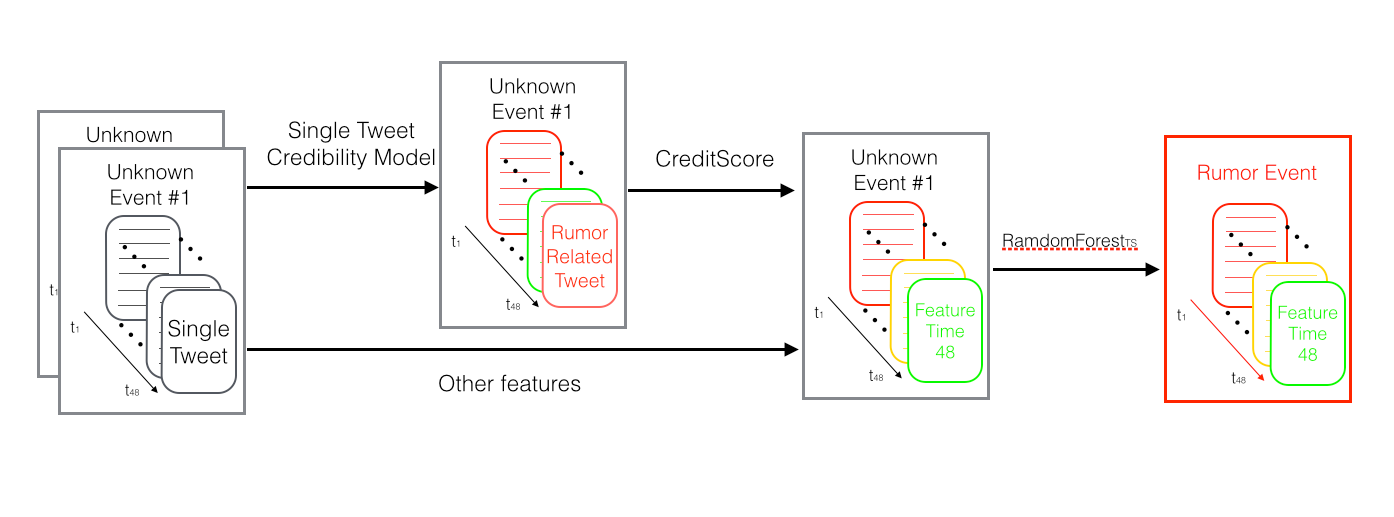
\includegraphics[width=\columnwidth]{images/structuremodel.png}
\caption{ pipeline of the rumor detecting system }
\label{fig:pipeline}
\end{figure}

 \newpage
 \subsection{Contributions}
In this thesis, we make the following contributions:

\begin{itemize}
	\item Our work is the first research which clearly defines the time period of rumor events. Other works either use natural time period (week or month) or do not explain their definition. We develop a novel approach for definition of rumor's time period in Section \ref{sec:Time_Period_of_an_Event}. 
	\item We develop a model for classifying single tweet with high credibility or low credibility. We call it \textsc{single tweet's creditability scoring model}. It is trained only with features which can be extracted from single tweet. We test 2 different kinds of models: classifier with handcrafted features and network models.   Single tweet's creditability scoring model gets 81\% accuracy.

 	\item We develop a time series model for detecting rumor events TS-RF. We used Dynamic Series-Time Structure (DSTS)\cite{liu2015real} to capture the temporal  features. And we use the parameters of 3 epidemiological models as features: modified SpikeM Model \cite{kwon2013prominent}, SIS model and SEIZ model \cite{jin2013epidemiological}. Within 48 hours after the event's spreading, TS-RF model can detect the rumor events with 90\% accuracy. 
 	\item  We add the outputs of single tweet's creditability scoring model as a feature into TS-RF, in order to improve the performance in the early stage. We call it CreditScore. And we approve that CreditScore is the best feature in the rumor detection task and it can significantly improve accuracy of rumor detection in first 24 hours.

 	\item We study how the performances of features change over time during the spreading of rumors. For example the performance of features about external URLs gets better after 24 hours and the features of sentiments are useless after 25 hours. And within 25 hours which is the average time for human editors detecting rumors, we get 87\% accuracy for rumor detection.

 \end{itemize}
 
 
\subsection{Thesis Outline}

The rest of this thesis is organized as follows: In Chapter~\ref{cha:Related_Work} we explain some terminology of Twitter and some techniques which we use for extracting feature and modeling. In Chapter~\ref{cha:single_tweet_creditbility_scoring_model}, we introduce our single tweet's credibility model. We show the performance of models with handcrafted features are worse than the neutral network model. In Chapter~\ref{cha:timr_seriers_rumor_model}, we introduce the time series model TS-RF and the time series features. We compare the time series model and static model and we discuss the performance of features changing over time. Finally, in Chapter~\ref{cha:conclusion_and_future_work} we add some concluding remarks and describe future work.

% chapter introduction (end)